\begin{pr}
Let $C_i$ denotes the instructor that will teach class $i$.
\begin{enumerate}[(1)]
\item
\begin{itemize}
\item Variables: $C_1, C_2, C_3, C_4, C_5$.
\item Domains: $C_1\in\{A, C\}, C_2\in\{A\}, C_3\in\{B, C\}, C_4\in\{B, C\}, C_5\in\{A, B\}$.
\item Constraints: $C_1\neq C_2, C_2\neq C_3, C_2\neq C_4, C_3\neq C_4$.
\end{itemize}
\item 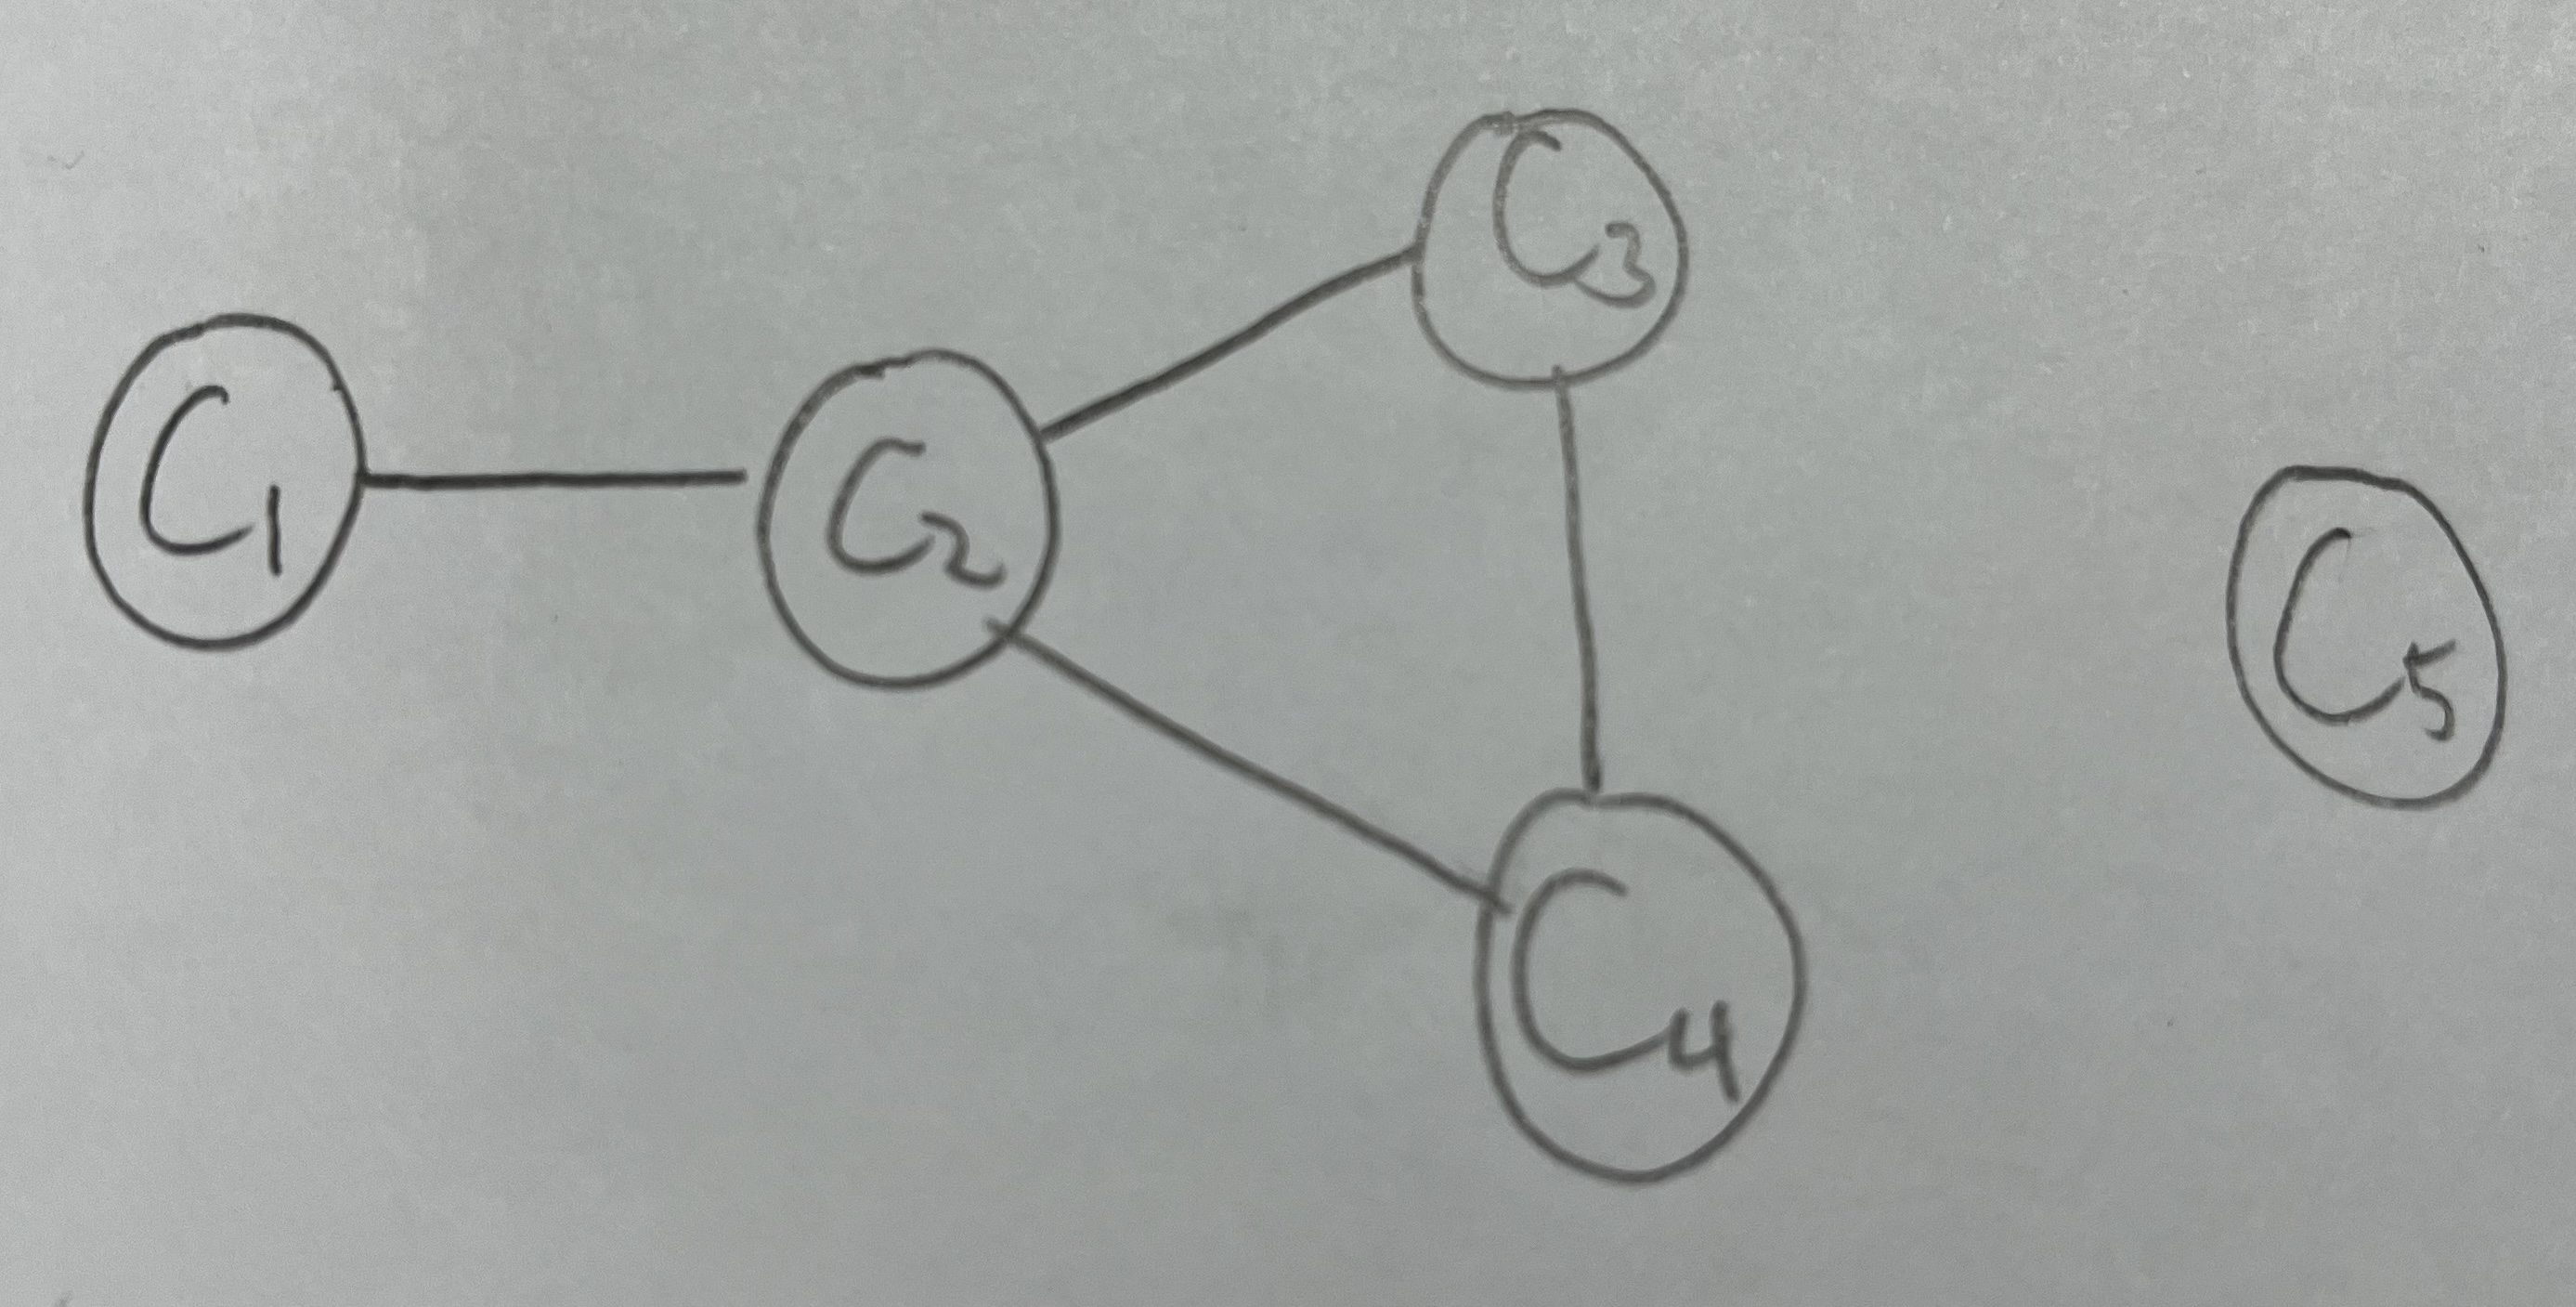
\includegraphics[width=7cm]{p3.JPG}
\item $C_2\in\{A\}\then C_2=A\then C_1\in\{A, C\}\setminus\{A\}\then C_1=C$.\\
New domains: $C_1\in\{C\}, C_2\in\{A\}, C_3\in\{B, C\}, C_4\in\{B, C\}, C_5\in\{A, B\}$.
\item $(C_1, C_2, C_3, C_4, C_5)=(C, A, B, C, B)$.
\item It is because one can solve a tree-structured CSP in $O(nd^2)$ (symbols same as ppt) time complexity, which is much faster than solving a general CSP.
\end{enumerate}
\end{pr}
\newpage
